%!TEX root = /Users/markelikalderon/Documents/Git/timaeus/timaeus.tex

\chapter{Psychogeny} % (fold)
\label{cha:psychogeny}

\section{Psychogeny and the Philosophy of Perception} % (fold)
\label{sec:psychogeny_and_the_philosophy_of_perception}

What is there to learn about the philosophy of perception from Timaeus' psychogeny? 

The Demiurge's procedure in the generation of the World-Soul falls into three parts. First, He generates the substance of the soul by mixing indivisible and divisible Being, Sameness, and Difference. Second, He establishes proportional divisions in the substance of the soul. And finally, from this substance, He fabricates the Circles of the Same and the Different. The structure of the soul and the materials from which it is fabricated determine its capacities. 

But what capacities are these? Ancient opinion divides. According to one view, associated with Xenocrates, the composition of the World-Soul explains the soul as the principle of motion. According to another, associated with his student Crantor, the composition of the World-Soul explains the soul as the principle of cognition. (For these views see Plutarch, \emph{De animae procreatione in Timaeo} 1012e--1013a.) While the details of Xenocrates' and Crantor's accounts are inconsistent with one another, the general claims that the soul is the principle of motion and that it is the principle of cognition are not, as Aristotle explicitly recognizes:
\begin{quote}
	For having constituted the soul out of the elements and having divided it accordance with the harmonic numbers so that it might have an innate perception of harmony and so that the whole universe might be borne in harmonious orbits, he bent the straight into a circle. (Aristotle, \emph{De anima} 1 406b28--31; \citealt[10]{Shields:2016ix})
\end{quote}
(The elements here are not the Empedoclean ``roots'', the four primary bodies---fire, air, water, and earth---but, rather, indivisible and divisible Being, Sameness, and Difference.) According to Aristotle, then, the composition of the World-Soul both explains why it cognizes harmony and moves the Cosmos in harmonious orbits. The composition of the World-Soul, on Aristotle's view, thus explains the soul as the principle of motion and the principle of cognition. Our focus shall be on the latter explanation.

Since the soul of mortal beings is constructed from the same materials, even if the mixture is less pure, with the same proportional divisions and structure, the soul of mortal beings at the very least have similar cognitive capacities. So an understanding of the psychogney promises to shed light on the cognitive capacities of mortal beings.

This is not yet to establish psychogeny's relevance to perception. Psychogeny may be relevant to the cognitive capacities of the immortal soul, but perception is linked, instead, to the mortal soul. But, as we shall see (chapter~\ref{cha:common_pathemata}), perception involves reporting its object to the \emph{phronimon}, the seat of cognizance. Timaeus conceives of perception as a kind of measurement. In perception, the sentient body is affected and this affection is the measure of the power of the agent that caused this affection. When this power is reported to the \emph{phronimon}, perception supervenes. Though elusive, the \emph{phronimon} is naturally understood as among the cognitive capacities of the immortal soul. The young gods may endow mortal beings with a mortal soul, in part, so that they may perceive, but the power to do so depends upon the cognitive capacities they have thanks to their immortal soul, an immortal soul constructed in a parallel fashion to the World-Soul. Indeed, as we shall see (chapter~\ref{cha:the_end_of_vision_and_audition}), Timaeus' sensory soteriology (47a--e) crucially depends upon this parallel.


% section psychogeny_and_the_philosophy_of_perception (end)

\section{Incarnation and Psychogeny} % (fold)
\label{sec:embodiment_and_psychogeny}

If cosmogeny describes the generation of the body of the Cosmos, psychogeny describes the generation of the World-Soul. Timaeus goes out of his way to point out that he treats these subjects out of order (34b11--35a1). We are not to suppose that the body of the Cosmos was created first and only then is the soul that animates it created. The World-Soul rules over the body of the Cosmos and it is only fitting that the elder should rule over the younger. If Timaeus' narrative departs from the natural order of things, this is solely due to human limitations in understanding such matters.

The psychogeny is not only preceded by the cosmogeny in Timaeus' speech, but it is also preceded by an account of the soul--body union (34a8–34b10). Timaeus concludes his account of the generation of the body of the Cosmos with an account of its ensoulment. Moreover, this account is repeated at the conclusion of the psychogeny (36d8--e5). Thus the Timaean psychogeny is bookended with accounts of the union of the body of the Cosmos with the World-Soul. Here, however, Timaeus does not remark about the oddity of his procedure. If one thinks about the all too human demands of exposition, would it not be more natural to give an account of the soul--body union only after giving accounts of the soul and the body? And why repeat the account of soul--body without apparent embellishment? 

Other puzzles, however, will be our central concern. The accounts of the ensoulment of the body of the Cosmos and the incarnation of the World-Soul ascribe spatial properties to the World-Soul, as does the psychogeny proper. However, these straightforwardly conflict. On the first, the World-Soul is stretched from the center throughout the body of the Cosmos so as to entirely encompass it. The World-Soul is thus depicted as a voluminous sphere. On the second, it consists in circles, the Circles of the Same and the Different, with the Circle of the Same containing the Circle of the Different, which is itself divided into smaller circles. On the second account, unlike the first, the World-Soul is not a voluminous sphere. What is more, each is internally incoherent. On the first account, the World-Soul is said to encompass the spherical body of the Cosmos. But beyond the limits of the Cosmos is neither space nor void. If beyond the limits of the body of the Cosmos there is neither space nor void, there is no space in which the World-Soul may encompass it. On the second account, the Circle of the Different is said to be contained within the Circle of the Same and so smaller than it, and yet each are produced from two strips of material of equal length. 

These puzzles do not admit of a proper resolution. There is no way to read the account of soul--body union and the psychogeny both literally and coherently. Moreover, these puzzles are so blatant and on the surface of the text that is not possible to read Timaeus as being unaware of them. On this basis, I shall argue that the ascriptions of spatial properties to the World-Soul cannot be interpreted literally. This, in turn, has an important consequence. Not only does Timaeus ascribe spatial properties to the World-Soul, but he also ascribes motion to it. But if we cannot interpret the ascription of spatial properties to the World-Soul literally, neither can we interpret the ascription of motion to it literally. 

% section embodiment_and_psychogeny (end)

\section{The Soul-Body Union} % (fold)
\label{sec:the_embodiment_of_the_world_soul}

Timaeus accounts for the union of the World-Soul and the body of the Cosmos twice over. And though there are minor differences in detail, there is no substantive embellishment in the second retelling. What, then, could justify the retelling? One thought might be that Timaeus does so for emphasis. After all, the soul--body union is an important topic. However, his account of the the union of the World-Soul and the body of the Cosmos is brief, much briefer and less involved that his account of the psychogeny proper. If emphasis was really Timaeus' concern, would not a more elaborate account be a better way to accomplish it? 

I suspect that the same Demiurgic activity is being described from two different perspectives. The Cosmogeny ends with a description of the ensoulment of the body of the Cosmos. Similarly, the psychogeny ends with a description of the incarnation of the World-Soul. Each describes the same event brought about by Demiurgic activity, though from the perspective of different participants of that event.

Timaeus describes the ensoulment of the body of the Cosmos at 34a8--34b10. Timae\-us begins by summing up, in reverse order, his discussion of cosmic morphology: The Demiurge has created the body of the cosmos with a smooth and even surface (33b8--34a8), with sides of equal distance from its center (33b4--8), a complete body made up of complete bodies (33b1--4). Now he describes what happens to it, the body of the Cosmos, as a result of Demiurgic activity. The Demiurge begins by placing soul in the center of the Cosmos. Note well the lack of a definite article. Timaeus does not say that that he placed the soul in the midst of the Cosmos, but soul (a detail keenly observed by Proclus, \emph{In Timaeum} 2 107, \citealt{Diehl:1903re}, though perhaps he owes this observation to Syrianus). The occurrence of \emph{psuchē}, here, is thus better interpreted as a mass noun rather than a count noun. This contrasts with the ensoulment of mortal beings. The soul of mortal beings is placed in the midst of their body, bound to marrow and encased by bone and flesh. Not so the World-Soul. Having placed soul in the middle of the body of the Cosmos, the Demiurge stretches (\emph{eteinen}) the soul throughout the whole of it. The World-Soul thus permeates the body of the Cosmos. There is a potential echo of Empedocles here: ``but it/he is only a sacred and ineffable thought organ darting through the entire cosmos with swift thoughts'' (DK 31B134, \citealt[263]{Inwood:2001ve}). Not only does the the World-Soul permeate the body of the Cosmos but it encompasses it from without, covering it all around (\emph{perikalupsen}). 

Proclus understands the imagery, here, as illuminationist. Soul having been placed in the center of the Cosmos illuminates by its powers the whole of the Cosmos and beyond (\emph{In Timaeum} 2 108, \citealt{Diehl:1903re}). If the aptness of the illuminationist imagery is unclear, compare Robert Grosseteste's vivid description of the propagation of light:
\begin{quote}
	For light of its very nature diffuses itself in every direction in such a way that a point of light will produce instantaneously a sphere of light of any size whatsoever, unless some opaque object stand in the way. (Robert Grosseteste, \emph{De luce}, \citealt[10]{Riedl:1942it})
\end{quote}
The retelling of this event, from the perspective of the World-Soul, invokes, in addition, a textile metaphor. Soul is said to be interwoven into the body of the Cosmos. The imagery in both passages, though distinct, need not conflict and may be complementary. Indeed, as we shall see, the weaving metaphor in the retelling potentially lends significance to the occurrences of \emph{eteinen} and \emph{periekalupsen} in the initial telling. Moreover, the illuminationist imagery arguably persists, the retelling simultaneously presenting, in a Joycean fashion, both images.

We are not to envision the World-Soul's encompassment of the body of the Cosmos as their merely being coincident. Rather, the World-Soul does so from without (\emph{exōthen}). \citet[58]{Cornford:1935fk} tries to resist this interpretation, claiming, instead, that the World-Soul is coincident with the body of the Cosmos (see also \citealt[105]{Taylor:1928qb}, \citealt[85]{Skemp:1942oc}, \citealt[70]{Robinson:1970lq}). He cites Alcinous as a precedent (\emph{Didaska\-likos} 14.4). There are two problems with this bit of evidence. First, there is no consensus among ancient commentators on this interpretation as Proclus reports (\emph{In Timaeum} 2 104--8, \citealt{Diehl:1903re}) And, second, Alcinous, there, seems to conflate the exterior portion of the World-Soul with the Circle of the Same in a way not borne out by the text (though see \citealt[105]{Taylor:1928qb}). Cornford, in addition, cites other occurrences of \emph{exōthen} such that, if the present occurrence is read in light of these, it would not carry the implication that the World-Soul extends beyond the body of the Cosmos. Cornford cites occurrences of \emph{exōthen} in Aristotle (``the parts of animals on the outside'', \emph{ta exōthen moria tōn zōōn}, \emph{Historia animalium} 494a22) and in Plotinus (``the circumference on the outside'' of a circle, \emph{hē exōthen periphereia}, \emph{Ennead} 2.2.1). Neither occurrence serves Cornford's purpose, however. Animals and corporeal circles exist in an environment which their outer surface or circumference faces. But the Cosmos does not itself exist in an environment. It is the environment. While it may have an inner circumference, it lacks an outer circumference. It is not outer facing since there is nothing outer to face. The only Platonic occurrence Cornford cites is \emph{Sophist} 253d where the specific Forms are embraced from the outside by the generic Form, remarking that ``the genus does not extend farther than the species it contains''. But the Forms are by nature a-spatial. There is no question of reading \emph{exōthen} as anything other than a metaphor here. This contrasts with the present case where it is very much an open question whether the spatial language that Timaeus uses to describe the World-Soul is best understood literally. And even if it is not, to discern its significance, we first must take it seriously. Thus, for example, Proclus, following his teacher Syrianus, takes the World-Soul to be non-coincident with the body of the Cosmos and understands its extending beyond the Cosmos in the \emph{eikos muthos} as indicating a hypercosmic aspect (\emph{In Timaeum} 2 105--6, \citealt{Diehl:1903re}).

If I am right, and we have to take seriously Timaeus' claim that the World-Soul encompasses the body of the Cosmos from without, then there is a puzzle here. Indeed, I suspect that Cornford's motivation for his alternative interpretation consists, in part, in the avoidance of this puzzle. Beyond the limits of the Cosmos is neither space nor void. There is no space, then, for the World-Soul to extend beyond the limits of the Cosmos. If we take the spatial language of \emph{exōthen} seriously, then there is no coherent way to understand it literally. What then is its significance? 

\citet[144--5]{OBrien:1969ty} sees here a Platonic criticism of Empedocles:
\begin{quote}
	The position of Plato's soul is the same as the position we have attributed to Love, stretching out from the centre in all directions in the form of a sphere. But Plato makes a point of wrapping soul round the \emph{outside} of the elements as well. This is very likely in order to make Love occupy the position of Strife. In this way Plato shows agains his denial of the existence of Empedocles' evil god, precisely as he had done in the \emph{Politicus}, and by slight implication in the Sophist. \citep[145]{OBrien:1969ty}
\end{quote}
O'Brien may well be right about this. Despite many points of contact between Timaeus' cosmogeny and Empedocles' (the Cosmos is composed of the four elements united by \emph{philia}, is spherical at least when Love dominates, and has no need for hands and legs), Strife is conspicuous in its absence. I doubt that the significance of the World-Soul encompassing the body of the Cosmos is exhausted by this criticism of Empedocles, however. I suspect that Timaeus is making a positive as well as a negative point. Soul's encompassment of the corporeal is meant, in addition, to mark a contrast between the ensoulment of the body of the Cosmos and the ensoulment of the bodies of mortal beings. Whereas the World-Soul encompasses the body of the Cosmos, the body of a mortal being encompasses its soul. We shall discuss this contrast further in chapter~\ref{cha:incarnation}.

The incarnation of the World-Soul is taken up after the completion of the psychogeny (36d8–e5). The ensoulment of the body of the Cosmos is now narrated from the perspective of the World-Soul, the other participant in the soul--body union. When the Demiurge completes the construction of the World-Soul to his satisfaction, He fabricates within it all that is corporeal. This marks the first difference with the ensoulment of the body of the Cosmos. According to that earlier narrative, soul is placed in the center of the Cosmos and is stretched throughout so as to encompass it from without. According to the present narrative, the encompassment of the body of the Cosmos from without is clear from the very beginning. The corporeal is generated within the World-Soul. Timaeus also adds a detail not present in the narrative of the ensoulment of the body of the Cosmos. There we were told that soul was placed in center of the Cosmos. When narrating the incarnation of the World-Soul, Timaeus claims, in addition that they are placed center to center. The new detail, then, is that the World-Soul has a center and that this is coincident with the center of the body of the Cosmos. A third difference is the introduction of textile imagery. Timaeus goes on to claim that the World-Soul is interwoven everywhere (\emph{pantē daiaplakeisa}) throughout the Heaven (\emph{ouranos}, here, used as equivalent to \emph{kosmos}) and encompassing it from without (\emph{exōthen perikalupsasa}). Proclus notes a fourth potential difference between our two passages:
\begin{quote}
	These things differ not at all from the words that are presently before us, for the phrases `extending it from the middle in every way' and `interwoven from the middle on out in every direction to the outermost edge of the heaven' come to the same thing except that in the one case [the retelling] the soul itself from itself has illuminated by its own powers the centre of the universe and the whole sphere, but in the present case [the initial telling] the Demiurge is the cause of the ensoulment when he transplants the soul into the universe. (Proclus, \emph{In Timaeum} 2 108, \citealt{Diehl:1903re}; \citealt[64]{Baltzly:2009bc})
\end{quote}
If Proclus is right, it is doubtful that Timaeus is denying Demiurgic agency in the retelling of the event. Rather, he is emphasizing that soul is the cause of intelligent and unceasing life of the Cosmos and that its body is a passive recipient of these.

The weaving metaphor is not incidental. It is invoked again and at greater length in Timaeus' discussion of the soul--body union of mortal beings (41d, discussed in chapter~\ref{sec:the_demiurge_addressing_the_gods}). Indeed, weaving imagery is not infrequent in the Platonic corpus (\emph{Theaetetus} 202b3, \emph{Sophist} 259e6, 262d4, \emph{Statesman} 279a--283a, and \emph{Cratylus} 387e--390b). The earlier occurrences of \emph{eteinen} and \emph{perikalupsen} are, perhaps, explicable in terms of the weaving metaphor now invoked. First consider \emph{eteinen}. In a loom the warp threads are stretched tight and used as support for the weft which is drawn through. The soul of the Cosmos, that within which its body is generated, seems analogous to the warp in the support in lends to the corporeal. This is why it is stretched tight throughout. Second, \emph{exōthen perikalupsasa} itself has textile connotations. Homer uses similar language to describe a cloak that surrounds a body as an image for sleep enveloping the sleeper (\emph{Illiad} 14.359). And a cloak is itself a product of weaving. The weaving imagery, more prominent in the retelling of the event than in its initial telling, need not be inconsistent will the illuminationist imagery that Proclus discerns (should it indeed be of genuine Timaean provenance). Indeed, if Timaeus is, in fact, in a Joycean fashion, simultaneously pursuing illuminationist and textile imagery, the former will constrain the interpretation of the latter. For example, \citet[406]{Cherniss:1944aa} observes that ``it is by understanding in a literal physical sense the `intertwining' of the soul with body (\emph{Timaeus} 36e) that [Aristotle] reduces Plato's account of the movement of body by soul to the mechanical propulsion of Democritus (\emph{De anima} 406b25--28)'' and complains that he thus misses out the way that soul's encompassment of body (34b, 36e) signals its special status. Cherniss might have mentioned as well that Aristotle's interpretation of weaving is inconsistent with the illuminationist imagery that Proclus sees Timaeus as simultaneously pursuing. Specifically, the literalist interpretation of the weaving metaphor where soul and the body it moves are spatially distinct is inconsistent with soul permeating body the way light seems to permeate the air.

% section the_embodiment_of_the_world_soul (end)

\section{Soul Mixture} % (fold)
\label{sec:soul_mixture}

The first step in the psychogney is the generation of the substance of the World-Soul from the mixture of indivisible and divisible Being, Sameness, and Difference. The dominant modern interpretation of this mixture (\citealt{Grube:1932qr}, \citealt[60--1]{Cornford:1935fk} \citealt[70--1]{Robinson:1970lq}) is due to Proclus, \emph{In Timaeum} 2 (\citealt{Diehl:1903re}, for discussion of alternative interpretations see \citealt[106--36]{Taylor:1928qb}, \citealt[51--54]{Shorey:1889sx}, and \citealt[352]{Shorey:1928ar}). According to the Proclean interpretation, the mixture occurs in four stages. Specifically, the Demiurge mixes:
\begin{enumerate}[(1)]
	\item indivisible and divisible Being
	\item indivisible and divisible Sameness
	\item indivisible and divisible Difference
	\item the three resulting mixtures (1--3)
\end{enumerate} 
We shall examine these in turn. But first let us consider the contrast between the indivisible and the divisible.

Timaeus marks a contrast between what is indivisible and what is divisible. With respect to indivisible (\emph{ameristou}) Being it is said to remain always the same (\emph{aei kata tauta}), whereas divisible Being is said specifically to be divided around bodies (\emph{peri ta somata} \ldots\ \emph{meristēs}) and becoming (\emph{gignomenēs}). Since \emph{gignomenēs} contrasts with \emph{aei kata tauta} presumably it means something like becoming or subject to change rather than being generated in the narrow sense of having come to be as the product of some agency. The associations of being changeless with the indivisible and being subject to change with the divisible presumably carry over to the application of this distinction to Sameness and Difference as well. Presumably so too does the specification of the divisible as being divided around bodies. The specification also provides a hint about the intended contrast. Recall that, for Timaeus, the mark of the corporeal is that it is sensible rather than being extended as it is for Descartes. This carries the strong suggestion that the indivisible is, by contrast, intelligible.

(1) \emph{Indivisible and divisible Being.} Being that is divided around bodies and subject to change is the kind of being suffered by the sensible and the corporeal. That much is clear. But what about indivisible Being? If we follow the suggestion that it is intelligible, then it is natural to suppose that it is the kind of Being enjoyed by the Forms. Individual Forms, it might be thought, are incomposite and hence indivisible (\citealt[64]{Cornford:1935fk}, \citealt[71]{Robinson:1970lq}). The corporeal objects of sense, by contrast, are composite. We learn that they are composed of elemental triangles themselves too small to be seen. (This is one of the two interpretations that Calcidius attributes to the ancients, \emph{In Timaeum} 2 29--31. On the alternative, indivisible Being is the kind of soul that resists embodiment, and divisible Being is the vegetative soul, common to all living beings, animals as well as plants, that animate these, and the mixture is the rational soul. This is a clearly Peripatetic take, and one that shows an Alexandrian influence.) One difficulty with this suggestion, perhaps not insurmountable, is that a prominent example of a changeless intelligible being in the \emph{Timaeus} is the Paradigm. But the Paradigm is a comprehensive living being that contains within itself all other intelligible living beings. If the Paradigm is indivisible it must be so in a sense consistent with its comprehensiveness. Thus \citet[64]{Cornford:1935fk} writes ``A Form may indeed be complex and definable; but it is not `composite' ({\sbl σύνθετον}), not `put together' out of parts that can be actually separated or dissolved.'' Thus so long as the intelligible living beings contained within the Paradigm are not separable parts that are put together to form the Living Being, its comprehensiveness is consistent with being indivisible in the relevant sense.

If the substance of soul is generated, in part, by mixing indivisible and divisible Being, then the point of this Demiurgic procedure must surely be to endow soul with affinities to each. While the body of the Cosmos is visible the World-Soul is invisible (36e8). In this respect it is like indivisible Being and unlike divisible Being. Moreover, the World-Soul permeates the body of the Cosmos. If this does not come to the same thing as being extended, at the very least it is present to every part of the Cosmic body. (I hedge only because being extended comes dangerously close to just being divided around bodies. After all, to be extended is to be partly here and partly there. For Platonically inspired accounts of soul's presence in body without being extended and so divided around the body see Nemesius \emph{De natura hominis} 3 and Augustine \emph{De immortalitate animae}. Each may have been drawing upon Porphyry who in turn drew upon Plotinus whose views were influenced by the \emph{Timaeus}.) In this respect it is like divisible Being and unlike divisible being. The World-Soul, though generated, at least according to the \emph{eikos muthos}, is imperishable like indivisible Being (since perishing is a kind of change and indivisible Being is changeless.) Nevertheless, its activities are variable. Among its activities is forming true opinions about what transpires in the sensible realm. These will vary as the sensible realm varies. In this respect, it is like divisible Being.

This last observations suggests a different if complementary take on the point of Demiurgic mixture. If Timaeus subscribes to the principle that like is known by like, then part of the point of mixing indivisible and divisible Being is so that the World-Soul may cognize each (see Aristotle, \emph{De anima} 404b16--18, 406b28--31, Alcinous \emph{Didaskalikos} 14.4). Indeed it is capable of both contemplating the intelligible, like its maker and Father, and opining about the sensible and the corporeal. As Shorey observes, the point generalizes:
\begin{quote}
	It is necessary that the Soul should recognize everywhere \ldots\ the \emph{same}, the \emph{other} and \emph{essence}, those three {\sbl μέγιστα γένη} of the \ldots\ \emph{Sophist}. Hence, on the Greek principle that like is known by like, Plato makes real substances out of these three abstractions and puts them as plastic materials into the hands of the Demiurgus for the formation of the Soul.
\end{quote}

(2) \emph{Indivisible and divisible Sameness.} If Forms are indivisible, in some suitable sense, and every Form is the same as itself, then the Forms enjoy a kind of indivisible Sameness. The sensible and the corporeal are divisible. And yet they too may, in some sense, remain the same. Though the pages of a book may yellow with age, it remains the same copy despite this variability. The sensible and corporeal thus suffer a divisible form of Sameness. If the indivisible form of Sameness enjoyed by Forms preclude their changing in any way, the divisible form of Sameness suffered by the sensible and the corporeal is consistent with a body undergoing change while remaining, in some sense, the same body (at least as long as the change in question is not the body's destruction).

What could the intermediary form of Sameness, produced by Demiurgic mixture, be? Again the Sameness of soul must share affinities with indivisible and divisible Sameness. The affinities with divisible Sameness are perhaps the clearest. Like the divisible Sameness suffered by the sensible and the corporeal, soul may remain the same despite a variation in its activities. So the intermediary form of Sameness is consistent with soul undergoing change, at least if a variation in activity counts as change. And with respect to the soul of mortal beings, which is composed of the same materials if less pure, the structure of the soul may be deformed as a result of the shock of embodiment in such a way that its capacities may be affected. Indeed they may be, temporarily at least, incapacitated. And yet there is a sense in which it is the same soul that suffers deformation and incapacitation. What then are the affinities this intermediary form of Sameness share with indivisible Sameness? Perhaps such an affinity is manifest in soul's independence from the corporeal. With respect to the World-Soul this is shown by the corporeal being generated within it, by its encompassment of the corporeal, and by its superiority in ruling the body of the Cosmos. While the bodies of mortal beings are not generated within their souls and are not encompassed by them but rather encompass them, like the World-Soul, the souls of mortal beings rule over the bodies they animate. An independence from the corporeal is also manifest in their remaining the same thoughout the process of \emph{metempsychosis}. If they did not, we could not meaningfully speak of reincarnation here.

(3) \emph{Indivisible and divisible Difference.} Not only is every intelligible Form the same as itself, but it differs from every other Form. I suspect that indivisible Being, Sameness, and Difference are coeval, that none take priority over the other. Thus part of what it is for an intelligible Form to enjoy indivisible Being is for it to be the same as itself. But equally, part of what it is for an intelligible Form to enjoy indivisible Being is for it be intelligibly differentiated from every other Form. Partly for this reason Plotinus describes the One as hyperontic. To be is to be intelligibly differentiated, at least in part, but intelligible differentiation implies a kind of plurality not suffered by the One (\emph{Ennead} 5). But what is distinctive about divisible Difference? If a sensible body may in some sense be the same despite suffering change, it must also be different from other sensible bodies. This difference is perhaps not as absolute as the indivisible Difference enjoyed by intelligible beings. Think of nutrition and the growth of mortal beings. Before consumption, nutriment is both external to and different from the mortal being that consumes it. After consumption, however, nutriment is transmuted into its blood and flesh and so is no longer external and different. Perhaps it is the fluidity of Difference among the sensible and the corporeal that earns the qualification of being divisible. That a sensible and corporeal being is different from every other sensible corporeal being is temporally indexed. At a given time it is different from every other body. But if bodies may gain parts from without, what was once different subsequently becomes the same. Another difference between indivisible and divisible difference might be this. There are no duplicate forms. No two Forms have exactly the same character. But there may be duplicates among the sensible and the corporeal that remain different despite having the same character.

Again, the intermediary form of Difference shares affinities with indivisible and divisible Difference. Just as the Forms are different from every other Form, souls are different from every other soul. Timaeus is no monopsychist. The souls of mortal beings do not partake of the World-Soul. The World-Soul is an elder sister to them, and is as different from them as mortal siblings are. In this way is the intermediary Difference like indivisible Difference. In what way is the intermediary form of Difference like divisible Difference? We speculatively illustrated divisible Difference in terms of gaining parts from without. But souls neither gain nor lose parts. What, then, is the affinity? Forms, being indivisible and changeless, have a fixed character. The character of a soul consists in its powers and activities. The activities of the World-Soul may vary. Its true opinions vary as the sensible varies. And not only do the activities of the souls of mortal beings vary, but so do their powers. These may be deformed or even incapacitated as the result of the shock of embodiment. No two Forms have exactly the same character. But two souls may have the same powers and activities, at least in principle. Indeed, Timaeus' sensory soteriology depends upon this. It is by intelligently deploying the powers of vision and audition that the souls of mortal beings may become like the World-Soul insofar as they can. Perhaps it is this departure from indivisible Difference that marks the affinity with divisible Difference.

(4) \emph{The resulting mixtures mixed.} The first three steps of generating the substance of the World-Soul consisted in the production of intermediary forms of Being, Sameness, and Difference by mixing indivisible and divisible forms of these. The fourth and final step consists in mixing these intermediary forms to produce the substance of the World-Soul. The World-Soul itself has not at this point been generated, only the substance from which it will be fabricated. Nor should substance here be understood as something like essence. It is rather the material from which the Demiurge, the craftsman god, will fabricate the World-Soul. Arguably, the proportional divisions that He imposes upon this substance are essential features of it, as are the strutures he fabricates, the Circles of the Same and the Different.

One interesting detail of the narrative concerns the recalcitrance of the mixture. The intermediary form of Difference resists being mixed with the intermediary form of Sameness. The Demiurge thus must deploy force in generating the final mixture. This is in a way to be expected, if Difference is opposed to Sameness. But why is Difference singled out as recalcitrant as opposed to Sameness and Difference mutually resisting their mixture? The narrative detail certainly signals an asymmetry in the opposition structure between Sameness and Difference, but I am uncertain as to its full significance.

% section soul_mixture (end)

\section{Proportional Division} % (fold)
\label{sec:proportional_division}

Having generated the substance of the World-Soul through mixture, the Demiurge straightaway sets about establishing proportional divisions within it. This occurs in three stages:
\begin{enumerate}[(1)]
	\item The Demiurge establishes a series of seven portions of the mixture consisting of an interlaced series of powers of two and three (the ``double intervals'' and the ``triple intervals'')
	\item Between these portions, the Demiurge inserts further portions corresponding to the harmonic and arithmetical means of the double and triple intervals
	\item Between portions that stand in a ratio of 4:3, the Demiurge inserts portions that correspond to 9:8
\end{enumerate}
Let us consider these in turn.

(1) First, the Demiurge establishes seven portions of the mixture. He seems not to be scoring proportional intervals into the substance of the World-Soul the way that a mason or carpenter might (\emph{pace} \citealt{Robinson:1970lq}). Rather, the language here suggests that Demiurge is taking certain portions of the mixture and using these to assemble, part by part, the World-Soul (or at least a preliminary state of it---the Demiurge will subsequently restructure it into the Circles of the Same and the Different). Later we learn that the substance of the World-Soul was mixed in a \emph{kratēr} (whose significance shall be discussed in chapter~\ref{sec:the_immortal_part}). So the image Timaeus presents us with is the Demiurge reaching into the \emph{kratēr} and drawing out portions of the mixture and assembling these into the substance of the World-Soul. Presumably these portions are held together by the proportions in which they stand, proportion being the fairest and most perfect of bonds (31c2–4, discussed in chapter~\ref{sec:the_elemental_composition_of_the_corporeal}).

The portions are assigned numerical values which, in the \emph{eikos muthos}, correspond to their relative magnitudes. Thus the Demiurge begins by taking a portion of the mixture and next takes a portion that is twice the amount of the first. The magnitude of the second portion is thus a power of two of the magnitude of the first. The relationship between the numerical values shifts in the third portion which Timaeus describes as half as much again of the second portion or three times as much of the first portion. So if the magnitude of the second portion is a power of two of the magnitude of the first, the magnitude of the third portion is a power of three of the first. And, in general, the seven portions constitute an interlaced series of powers of two and three:
\begin{center}
	\begin{tabular}{l l}
		\emph{First portion} & 1\\
		\emph{Second portion} & 2 (= 2\( ^1 \))\\
		\emph{Third portion} & 3 (= 3\( ^1 \))\\
		\emph{Fourth portion} & 4 (= 2\( ^2 \))\\
		\emph{Fifth portion} & 9 (= 3\( ^2 \))\\
		\emph{Sixth portion} & 8 (= 2\( ^3 \))\\
		\emph{Seventh portion} & 27 (= 3\( ^3 \))\\
	\end{tabular}
\end{center}
There is a tradition, dating from the Old Academy (Plutarch attributes it to Crantor, \emph{De animae procreatione in Timaeo} 1027d), of graphically representing the two series, of powers of two and three respectively, as two sides of a lambda:
\begin{center}
	\begin{tabular}{c c c c c c c}
		 & & & \( 1 \) & & &\\
		 & & \( 2 \) & & \( 3 \) &\\
		 & \( 4 \) & & & & \( 9 \)\\
		 \( 8 \) & & & & & & \( 27 \)
	\end{tabular}
\end{center}
Thus the powers of two are arrayed on the left hand side of the lambda while the powers of three are arrayed on the right hand side. 

One inteteresting arithmetical fact about this series, that suggests a Pythagorean influence, is that 27 is the sum of all of its predecessors:
\[
	1 + 2 + 3 + 4 + 9 + 8 = 27
\]

Many commentators represent the numerical values of these portions in ascending order:
\begin{center}
	\( 1 \) \( 2 \) \( 3 \) \( 4 \) \( 8 \) \( 9 \) \( 27 \)
\end{center}
While sensible for many purposes it does elide an odd feature of the account, namely that the fifth portion is larger than the sixth since the series of powers of three grow at a greater rate than the series of powers of two. If, however, the Demiurge is arranging the portions in the order narrated by Timaeus, then the portion eight times the size of the initial portion is placed in the substance of the World-Soul before the portion nine times the size of the initial portion in which case the numerical values should be ordered as follows:
\begin{center}
	\( 1 \) \( 2 \) \( 3 \) \( 4 \) \( 9 \) \( 8 \) \( 27 \)
\end{center}
Which does Timaeus intend?

The matter is unclear, and not to be settled by the present passage alone. For now, however, observe how this might be connected with the underlying image that Timaeus is working with. Earlier, I mentioned how many commentators think of the Demiurge as scoring proportional divisions in the substance of the World-Soul the way a carpenter or mason might. Notice, on this model, the numerical values represent distance between the intervals, rather than the magnitude of the portions. If the numerical values represent distance between the intervals, then they should appear in ascending order. If, however, the numerical values represent the magnitudes of the portions, there is no obstacle to the Demiurge placing a portion eight times as great as the initial portion after the portion nine times as great as the initial portion. 

(2) Having established proportional divisions within the substance of the World-Soul corresponding to the interlaced series of powers of two and three, the Demiurge now begins to fill in harmonic and arithmetical means between these. Like the elemental composition of the body of the Cosmos, where fire and earth were united by two means (chapter~\ref{sec:the_elemental_composition_of_the_corporeal}), the double and triple intervals are themselves united by two means. Recall, that two means were required to unite fire and earth in order for the body of the Cosmos to be a three dimensional voluminous whole. Why are two means required to unite adjacent portions of the seven selected by the Demiurge?

The harmonic and arithmetic means are filled in between the two series of the power of two and three. Let \( H \) be a harmonic mean and \( A \) be an arithmetical mean, then the series for the powers of two would be:
\begin{center}
	\( 1 \) \( H \) \( A \) \( 2 \) \( H \) \( A \) \( 4 \) \( H \) \( A \) \( 8 \) 
\end{center}
and for the powers of three it would be:
\begin{center}
	\( 1 \) \( H \) \( A \) \( 3 \) \( H \) \( A \) \( 9 \) \( H \) \( A \) \( 27 \)
\end{center}
A harmonic mean, \( H \), of two numbers, \( x_{1}, x_{2} \), can be represented as:
\[ H = \frac{2x_{1}x_{2}}{x_{1} + x_{2}} \]
Whereas, an arithmetic mean, \( A \), of two numbers, \( x_{1}, x_{2} \), can be represented as:
\[ A = \frac{x_{1} + x_{2}}{2} \]
Where \( x_{1} = 1 \) and \( x_{2} = 2 \) the harmonic mean \( H \) then would be \( \frac{4}{3} \) (or 4:3), and the arithmetic mean \( A \) then would be \( \frac{3}{2} \) (or 3:2). Thus, the series of the powers of two (in boldface) with the harmonic and arithmetic means filled in and reduced would be:
\begin{center}
	\( \mathbf{1} \) \( \frac{4}{3} \) \( \frac{3}{2} \) \( \mathbf{2} \) \( \frac{8}{3} \) \( 3 \) \( \mathbf{4} \) \( \frac{16}{3} \) \( 6 \) \( \mathbf{8} \)
\end{center}
And the series of the powers of three (in boldface) with the harmonic and arithmetic means filled in and reduced would be:
\begin{center}
	\textbf{1} \( \frac{3}{2} \) \( 2 \) \textbf{3} \( \frac{9}{2} \) \( 6 \) \textbf{9} \( \frac{27}{2} \) \( 18 \) \textbf{27}
\end{center}
If we bracket the issue about the ordering of the portions (whether or not the portion that receives the numerical value nine precedes the portion with the numerical value eight), and combine our two series with the harmonic and arithmetic means filled in, and drop any duplicates, we get the series (with the numerical values of the original seven portions in boldface):
\begin{center}
	\( \mathbf{1} \) \( \frac{4}{3} \) \( \frac{3}{2} \) \( \mathbf{2} \) \( \frac{8}{3} \) \( \mathbf{3} \) \( \mathbf{4} \) \( \frac{9}{2} \) \( \frac{16}{3} \) \( 6 \) \( \mathbf{8} \) \( \mathbf{9} \) \( \frac{27}{2} \) \( 18 \) \( \mathbf{27} \)
\end{center}

One final remark about the ordering of the original seven portions. The question is whether or not the portion associated with nine precedes the portion associated with eight. Notice that eight belongs to the series of powers of two, and nine belongs to the series of powers of three. Since the harmonic and arithmetic means were calculated within these distinct series, the relative ordering of these portions do no effect the calculation of the values of the harmonic and arithmetic means. And since eight and nine are adjacent in the final series, switching their relative order would not disrupt the overall structure of the series. So we so far have no decisive reason to favor eight preceding nine or nine preceding eight.

So far we have only been discussing the purely ``formal'' aspect of this stage of the proportional division of the substance of the World-Soul. Let us now consider the ``material'' aspect of the \emph{eikos muthos}. What, according to Timaeus' myth, is the Demiruge doing exactly? Having taken seven portions of the mixture from the \emph{kratēr} and ordered them, the Demiurge cuts off further portions from the mixture corresponding to the harmonic and arithmetic means and sets them between the original seven portions. The series of rational numbers that we have arrived at must be the magnitudes of these portions. They could not be a measure of the distance between intervals the way the would be if they were scored in the substance of the World-Soul in the manner of the carpenter or a mason. Consider the initial sequence of the series of powers of two:
\begin{center}
	\( \mathbf{1} \) \( \frac{4}{3} \) \( \frac{3}{2} \) \( \mathbf{2} \)
\end{center}
This was ``materially'' generated in the following fashion. The Demiurge cuts off an initial portion of the mixture. He then cuts off another portion of the mixture twice that of the first. Now between these He places a portion four thirds of the first, the harmonic mean, between the first and the second and another portion three seconds of the first, the arithmetic mean, between the harmonic mean and the second portion. If the first and second portions of the original seven were initially adjacent, in inserting two further portions between them, the distance relations would change. So the rational numbers associated with the portions could not represent the distance between intervals, like the frets of a guitar. After all, their distance relations shift. The rational numbers could only represent their relative magnitude.

(3) The Demiurge is not yet finished with establishing proportional divisions within the substance of the World-Soul. In the series: 
\begin{center}
	\( \mathbf{1} \) \( \frac{4}{3} \) \( \frac{3}{2} \) \( \mathbf{2} \) \( \frac{8}{3} \) \( \mathbf{3} \) \( \mathbf{4} \) \( \frac{9}{2} \) \( \frac{16}{3} \) \( 6 \) \( \mathbf{8} \) \( \mathbf{9} \) \( \frac{27}{2} \) \( 18 \) \( \mathbf{27} \)
\end{center}
some of the intervals stand in the ratio of 4:3. Thus the interval between 1 and \( \frac{4}{3} \) stands in the ratio of 4:3 obviously, as does the interval between \( \frac{3}{2} \) and 2, and the interval between 3 and 4. In this third and final stage of this process, between portions that stand in a ratio of 4:3, the Demiurge inserts further portions of the soul mixture that correspond to \( \frac{9}{8} \) of the predecessor. Thus the ratio between 1 and \( \frac{4}{3} \) is 4:3, and so between these He inserts a portion of \( \frac{9}{8} \). With the insertion of new portions, we get new intervals, and this raises the possibility of iterating the procedure. And indeed we can, though not indefinitely. So consider the series:
\begin{center}
	\( \mathbf{1} \) \( \frac{9}{8} \) \( \frac{81}{64} \) \( \frac{4}{3} \)
\end{center}
\( \frac{81}{64} \) is nine eighths of its predecessor but if we try to introduce a new interval nine eighths of \( \frac{81}{64} \) we get \( \frac{729}{512} \) which is greater than \( \frac{4}{3} \). Here the Demiurge introduces ``leftover'' number, \( \frac{256}{243} \). Notice, this is the number by which \( \frac{81}{64} \) can be multiplied so as to yield \( \frac{4}{3} \). So we get:
\begin{center}
	\( \mathbf{1} \) \( \frac{9}{8} \) \( \frac{81}{64} \) \( \frac{256}{243} \) \( \frac{4}{3} \)
\end{center}
In summary, the Demiurge's procedure then is this. Between portions whose numerical values stand in the ratio of 4:3, He inserts two portions nine eighths of its predecessor followed by a portion corresponding to the ``leftover'' number.

This three stage procedure exhausts the available supply of soul mixture. What is used up is not indivisible and divisible Being, Sameness, and Difference. More remains and will be used to generate the immortal part of the soul of mortal beings. What is used up is the mixture of these. The Demiurge has only stopped introducing proportional divisions since He has used up His supply of soul mixture. This is further evidence that the numerical values represent magnitudes of the portions of soul mixture as opposed to distance relations among the intervals they introduce. If the Demiurge was scoring proportional divisions into the substance of the World-Soul in the manner of a carpenter or mason, there is no reason why the subdivision could not continue indefinitely. But if the numerical values represent instead the magnitudes of the portions then His procedure naturally comes to an end when all of the soul mixture is used up.

% section proportional_division (end)

\section{The Circles of the Same and the Different} % (fold)
\label{sec:the_circles_of_the_same_and_the_different}

Having first generated the soul mixture from indivisible and divisible Being, Sameness, and Difference, and established proportional divisions in the substance of the World-Soul, the Demiurge now begins to fabricate the structure of the World-Soul. Specifically, from the soul mixture in which He has established proportional divisions, the Demiurge now constructs the Circles of the Same and the Different.

Timaeus first tells us that the Demiurge splits the assembled portions lengthwise. The assumption, here, is that the soul mixture in which the proportional divisions has been established is in rectilinear form. This is a natural consequence of the manner in which the Demiurge established these proportional divisions. Recall, He first cuts off seven portions of the soul mixture and apportions them more or less in order of ascending magnitude. (Recall, perhaps the portion eight times as great as the first precedes the portion nine times as great as the first.) Between these He places further portions corresponding to harmonic and arithmetic means. Finally, between portions in the ratio of 4:3, He places two portions of nine eighths of the preceding and a portion corresponding to a ``leftover'' number. If we consider the ``material'' aspect of this procedure, it results im a linear sequence of portions of rational magnitudes in (perhaps roughly) ascending order---in other words, a strip, which the Demiurge now proceeds to split lengthwise.

In splitting the proportionally divided mixture lengthwise, the Demiruge has made two strips. He now places them center to center to form the Greek letter chi, {\sbl Χ}. As Timaeus makes subsequently clear (39a1), these two strips are placed at oblique angles. There is no reason to suppose that they are initially placed at right angles and only subsequently moved as \citet[147]{Taylor:1928qb} and \citet[36 n1]{Bury:1929jb} suppose. After all, Timaeus omits this step from his narration. Taylor and Bury only infer it from the oblique motion described at 39a1. In addition, Proclus (\emph{In Timaeum} 2 238, \citealt{Diehl:1903re}) claims that the obliqueness of the angle follows from Timaeus' initial description. A chi, {\sbl Χ}, differs in form from, say, the multiplication sign, ×, not just in size but in that the strokes are set at oblique angles (see also \citealt[111 n7]{Archer-Hind:1888qd}). \citet[147 n1]{Taylor:1928qb} dismisses Proclus' observation claiming that it ``only shows that in the fifth century \textsc{A}.\textsc{D}. the [strokes] of the letter Chi were regularly oblique to one another''. \citet[67]{Jeffrey:1961aa}, however, in a survey of Greek inscriptions, reports that a chi with oblique strokes was normal in Attic script as far back as the sixth century \textsc{BCE}, though this admitted of frequent exceptions. Having set the strips center to center and at oblique angles, the Demiurge now bends these and joins each end to end to form inner and outer circles. 

Why circles? Timaeus has already proffered an explanation: because circular motion is most appropriate for reason and intelligence (34a, \citealt[31]{Vlastos:1975aa}). And in interweaving the body of the Cosmos with the World-Soul, the Demiruge invests it with reason and intelligence. Why circular motion is most appropriate for reason and intelligence shall be discussed in section~\ref{sec:the_cognitive_significance_of_circular_motion}.

There is a puzzle here about Timaeus' spatial language. While it has not gone wholly unnoticed, its full significance remains underappreciated. In what sense could the circles so much as be inner and outer? Recall, the Demiurge began by splitting the rectilinearly apportioned soul mixture lengthwise. Notice that the result of this procedure would be two strips of equal length. The result of producing two circles by bending them and joining each end to end would then be two circles of equal diameter. But the inner circle should have a smaller diameter than the outer circle. How could this be?

If we hang on to the idea that the circles are the result of strips of equal length and so of equal diameter, perhaps the puzzle may be mitigated by reflecting on the incorporeal nature of soul. The sensible is the mark of the corporeal and soul is invisible (36e8). If soul is invisible and hence incorporeal it is also intangible. And if soul is intangible, then it is not solid. (Recall that solidity is a condition on the possibility of touch, chapter~\ref{sec:the_elemental_composition_of_the_corporeal}.) If the two circles of soul mixture are not solid in the sense presupposed by the tangibility of the corporeal, they offer no resistance to one another and so may coherently interpenetrate as they would have to if they were of equal diameter and formed from strips that meet center to center. \citet[111--2 n7]{Archer-Hind:1888qd} and \citet[148]{Taylor:1928qb} give interpretations of this kind. Taylor describes them as geometrical circles on the surface of the celestial globe. But, of course, geometrical circles, being incorporeal, may interpenetrate. This line of reasoning is fine as far as it goes, but in what sense is one of the circles inner and the other outer? While a coherent account of the two circles may have been provided, it is an account inconsistent with a literal interpretation of Timaeus' spatial language. It is telling that \citet[112 n3]{Archer-Hind:1888qd} says that the one circle is outer in the sense of being superior thus investing ``outer'' with a non-literal significance.

Cornford senses the tension here, but his remarks on the passage are puzzling:
\begin{quote}
	The Demiurge takes a band of some pliable stuff, cuts it lengthwise into two strips, makes them touch at their middles and bends them round to form two rings, inclined to one another. \ldots\ One expression, in particular, is appropriate only to a material model: the second ring or ``circle'' is said to be ``inside'' the other. Plato is not imagining strictly geometrical circles, such as would appear on the surface of a celestial globe, for these would have the same diameter. But in a material model, made (say) of copper bands, one band would naturally be fastened ``inside'' the other. \citep[74]{Cornford:1935fk}
\end{quote}
While Archer-Hind endorsed a formal model positing strictly geometrical circles, Cornford recommends, instead, a material model. Indeed, it is partly for this reason that he likens the present construction to an armillary sphere (see figure~\ref{fig:2}). But a material model is precisely what could not be coherently maintained here. If the band of pliable stuff is cut lengthwise into two strips, then these strips will be of equal length. If these are now joined end to end, they will form circles of equal diameter. If we did this with copper bands, the inner band would be deformed to make room for the outer. But surely this would be an unwelcome asymmetry. Indeed in Timaeus' account of the shock of embodiment, such deformation is associated with rational incapacitation. Are we to imagine that the Demiurge did some unspoken work to avoid this unwelcome result? Perhaps He did not strictly join the inner band end to end but allowed it to overlap somewhat to form a circle with a smaller diameter than the outer circle. But this too would be an unwelcome asymmetry. Moreover, it departs from the text. Did He somehow work the inner band, pounding it out or in some other manner stretching it horizontally so as to shorten it? If so, why does Timaeus omit this important detail from his narrative? I am inclined to agree with Cornford that Timaeus is presenting us with a ``material model'' of the Demiurgic procedure, but, again, it is precisely such a model that is the source of the incoherence. Specifically, the apparent puzzle is only genuine if we insist upon a literal interpretation of the spatial attributes of the World-Soul.

\begin{figure}[htbp]
     \centering
         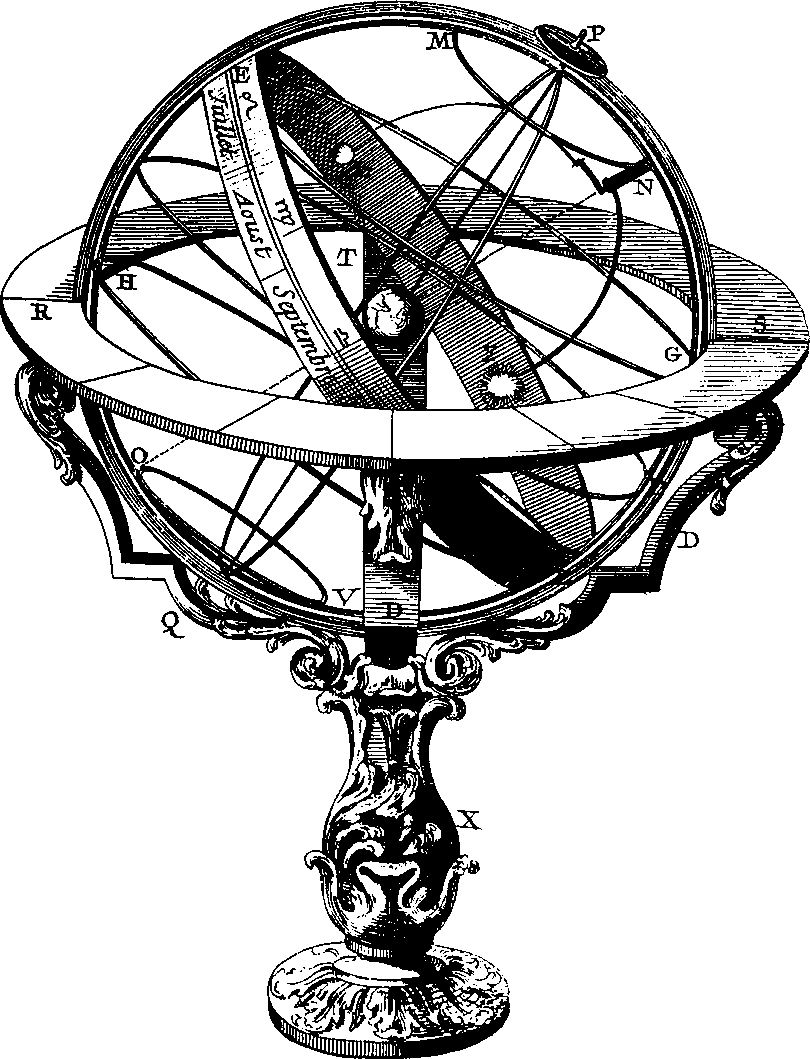
\includegraphics[scale=0.20]{graphics/Armillary_sphere.png}
     \caption{Illustration of an armillary sphere from Diderot's \emph{Encyclopédie}}
     \label{fig:2}
\end{figure}

Having fashioned the inner and outer circles, the Demiurge proclaims the outer circle to be the Circle of the Same and the inner circle to be the Circle of the Different and invests the whole construction with motion. Each circle rotates in place though in different directions:
\begin{enumerate}[(1)]
	\item The Circle of the Same, the outer circle, moves ``to the right and to the side''
	\item The Circle of the Different, the inner circle, moves ``to the left and along the diagonal''
\end{enumerate}
The motions of the World-Soul are the source of the motion of the body of the Cosmos. Thus the diurnal motion of the fixed stars is explained by the motion of the Circle of the Same, as the motion of the wanderers are explained by the motion of the Circle of the Different.

This presupposes a reading of {\sbl καὶ τῇ κατὰ ταὐτὰ ἐν ταὐτῷ περιαγομένῃ κινήσει πέριξ αὐτὰς ἔλαβεν} (36c3--4) that we have tacitly accepted. Most commentators understand this distributively, as describing the rotation in place of each of the circles. \citet[112 n2]{Archer-Hind:1888qd}, by contrast, seems to understand the claim of this passage collectively, and so as describing the motion of the whole construction, in which case Timaeus has described three motions: the motion of the whole and the motions of the two parts, the Circles of the Same and the Different. Whether or not the Greek can support the collective reading, it raises some difficulties that favor the conventional distributive reading. Are we to imagine that the Cosmos is subject to two rotational movements compounded out of the rotation of the whole and the rotation of the the Circle of the Same? Depending upon their speed and direction, these may cancel one another out. Are we to suppose instead that the alleged description of the motion of the whole is really just a description of the motion of the Circle of the Same? Then Timaeus has given redundant descriptions of the same motion. But why would he do that? For these reasons the claim is best understood distributively, as describing the rotation in place of each of the circles.

(1) The Circle of the Same is the outer circle. Timaeus claims that it moves ``to the right and to the side''. Timeaus' meaning is not immediately clear. Part of the problem is that we have not been given an explicit frame of reference, so it is unclear what to the right means. Timeaus' cosmology is geocentric. If we imagine the axis running through the North and South poles extending to the outer circumference of the Cosmos, then, for an observer looking South, movement to the right would be movement from East to West (\citealt[112--3 n5]{Archer-Hind:1888qd}, \citealt[150]{Taylor:1928qb}, \citealt[34 n23]{Vlastos:1975aa}; though see \citealt[122]{Dicks:1970aa}, and Plato makes the opposite assumption and imagines a North-facing observer in \emph{Laws} 760d). Taylor claims that this choice of frame of reference is justified since an observer in the Northern hemisphere, as the Greeks were, would have to face South in order to observe the path of the Sun in its entirety. \citet[74]{Cornford:1935fk} cites Proclus (\emph{In Timaeum} 2 258, \citealt{Diehl:1903re}) offering an alternative, if complementary, justification. In the Pythagorean table of opposites (Aristotle, \emph{Metaphysica} 985a22, see also \emph{Metaphysica} 1004b27ff, 1093b11, \emph{Ethica Nicomachea} 1106b29, \emph{Physica} 201b25), right is in the column of superior things and it is appropriate to ascribe a superior movement to the Circle of the Same since it rules over the Circle of the Different. That the movement to the right is to the side as well is emphasizing that the movement is taking place in the equatorial plane, again imagining this to extend throughout the entire Cosmos, and thus as the sidereal equator. 

% According to Vlastos, the movement of the Circle of the Same:
% \begin{quote}
% 	\ldots\ runs through the whole universe: everything in the cosmos, from its extreme periphery down to the center of our earth, is subject to this motion, though this is counteracted by other motions everywhere except in the region of the fixed stars. \citep[32]{Vlastos:1975aa}
% \end{quote}
% \citet[76]{Cornford:1935fk} had earlier made a similar claim and it will be later echoed by \citet[21--22 n26]{Zeyl:2000cs}. This presupposes a reading of {\sbl καὶ τῇ κατὰ ταὐτὰ ἐν ταὐτῷ περιαγομένῃ κινήσει πέριξ αὐτὰς ἔλαβεν} (36c3--4) that we have tacitly accepted. Most commentators understand this distributively, as describing the rotation in place of each of the circles. And Vlastos' claim that the motion of the Circle of the Same extends downwards to the center of the Cosmos is perhaps picking up on \emph{kata} here. \citet[112 n2]{Archer-Hind:1888qd}, by contrast, seems to understand the claim of this passage collectively, and so as describing the motion of the whole construction, in which case Timaeus has described three motions: the motion of the whole and the motions of the two parts, the Circles of the Same and the Different. Read collectively, Vlastos' claim becomes puzzling. Are we to imagine that the Cosmos is subject to two rotational movements compounded out of the rotation of the whole and the rotation of the the Circle of the Same? Depending upon their speed and direction, these may cancel one another out. Are we to suppose that the alleged description of the motion of the whole is really just a description of the motion of the Circle of the Same? Then Timaeus has given redundant descriptions of the same motion. But why would he do that?
%
% These difficulties do not arise on the distributive reading, and Vlastos' claim is best understood as resting upon this more conventional reading. However, it is worth noting that the justification that he explicitly offers for his claim is subject to criticism independently of how we read this passage (36c3--4). \citet[32 n14]{Vlastos:1975aa} justifies his claim, that the motion of the Circle of the Same extends from the circumference of the Cosmos to its center, noting that the World-Soul is everywhere interwoven in the body of the Cosmos (36e2--3). However, not only is that spatial description incoherent (since the World-Soul was said to extend into a region where there was neither space nor void), but, as we shall see, that spatial description of the World-Soul is inconsistent with the present description as well. If that is right, then Vlastos' justification is no justification at all. His claim that the motion of the Circle of the Same extends to the center of the Cosmos may yet be true for all that.

(2) The Circle of the Different is the inner circle. Timaeus claims that it moves ``to the left and along the diagonal''. Again his meaning is not immediately clear. The lack of an explicit frame of reference is a source of unclarity. If we assume, with Archer-Hind, Taylor, and Vlastos, that the implicit frame of reference is that of a South-facing observer, then movement to the left would be movement from West to East. What are we to make of its leftward movement, from West to East, being on the diagonal? We know that the strip of soul mixture from which the inner circle was formed was placed at an oblique angle to the strip from which the outer circle was formed. That much at least insures that it is not in the sidereal equatorial plane but intersects it diagonally. But in which direction?

The Tropic of Cancer is the Northern-most latitude of the Earth in which the Sun may be directly overhead. The Tropic of Capricorn, by contrast, is the Southern-most latitude of the Earth in which the Sun may be directly overheard. The sidereal planes that correspond to these bound the diagonal movement. The diagonal movement corresponds to the ecliptic, the Sun's Eastward movement through the Zodiac over the course of the solar year. The ecliptic is so-called since it is the only path through which eclipses may occur. The equinoxes are the points where the ecliptic intersects with the equator. If the diagonal is correctly identified with the ecliptic, then the diagonal is a sidereal plane from the Southwest to the Northeast bounded by the Tropics of Cancer and Capricorn. (While a reasonable approximation, the Sun in fact appears to trace a sinusoidal path across the sidereal equator.)

The Circle of the Same is granted sovereignty over the the Circle of the Different. Its rule is not grounded in in its substance which it shares with the Circle of the Different. Nor is it grounded in its proportional divisions which it shares as well with the Circle of the Different. We have seen \citet[112 n3]{Archer-Hind:1888qd} link its sovereignty to its being the outer circle, and Proclus (\emph{In Timaeum} 2 258, \citealt{Diehl:1903re}) with its movement to the right. But what Timaeus explicitly says is that in granting sovereignty to it, the Demiurge does not divide it the way He divides the circle of the Different. That is, Timaeus makes a claim about the consequences of granting sovereignty to the Circle of the Same and not about what merits that sovereignty. If we accept that the motion of the Circle of the same extends downwards to the center of the Cosmos, then its sovereignty is manifest in its moving the whole of the Cosmos \citep[76]{Cornford:1935fk}.

The Circle of the Same remains undivided so that it may rule over the Circle of the Different, but the subject of its rule is not exempt from such treatment. Specifically, the Circle of the Different is divided in six places so as to give rise to seven unequal circles. The divisions correspond to the powers of two and three. Timaeus claims that the three of the divisions occur at double intervals and three occur at triple intervals. The seven circles correspond to the initial seven proportional divisions of the substance of the World-Soul:
\begin{center}
	\( 1 \) \( 2 \) \( 3 \) \( 4 \) \( 9 \) \( 8 \) \( 27 \)
\end{center}
So the double intervals are the initial boundaries of portions of soul mixture whose magnitude corresponds to a power of two and the triple intervals are the initial boundaries of portions whose magnitude corresponds to a power of three. Perhaps this correspondence is something other than identity. Perhaps, that is, the diameters of these circles is simply a function of these values rather than measured by these values themselves. These circles correspond to the orbits of the planets, the wanderers. So perhaps the diameter of the Moon's revolution corresponds to one and the diameter of the Sun's revolution corresponds to two. Besides the Sun and the Moon, the Greeks recognized five planets: Venus, Mercury, Mars, Jupiter, and Saturn. The diameters of their orbits would correspond to the remaining five values of the initial seven proportional divisions.

It is unclear how the seven circles into which the Circle of the Different is divided are related to one another. Taking the solar system as a model, as we understand it to be, it is tempting to think of them as arranged concentrically. But Timaeus does not explicitly say so, and the assumption risks anachronism.

Timaeus does however tell us something about the relative speeds of their rotation. Three revolve at an equal speed. These correspond to the revolutions of the Sun, Venus, and Mercury. Four revolve at speeds neither equal to each other or with the three of equal speeds. These correspond to the revolutions of the Moon, Mars, Jupiter, and Saturn. While unequal in speed in these ways, Timaeus reports that their speeds stand in ratios equal to natural numbers.

As we have seen, there is a puzzle about Timaeus' spatial description of the Circles of the Same and the Different. Specifically, if the circles are generated from cutting the rectilinear apportioning of soul mixture lengthwise, this would result in strips of equal length and hence circles of equal diameter. But in what sense, then, could one be outer and the other inner? Suppose the seven circles into which the Circle of the Different is divided are in fact arranged concentrically. These would be encompassed by the Circle of the Same, and so the Circle of the Different would be inner, even on a literal understanding of that claim. One problem with this solution is that the Demiurge deems the outer circle as the Circle of the Same and the inner circle as the Circle of the Different before He divides the latter.

There is another puzzle about Timaeus' spatial language. This second puzzle concerns less the internal coherence of his spatial description of the Circles of the Same and the Different, than with how, if at all, it coheres with the spatial descriptions of the World-Soul given his accounts of the ensoulment of the body of the Cosmos (34a8--34b10) and the embodiment of the World-Soul (36d8--e5) (discussed in section~\ref{sec:the_embodiment_of_the_world_soul}). A common feature of these accounts is that the World-Soul is said to extend throughout the body of the Cosmos so as to encompass it from without. Bracket for the moment, our earlier puzzlement about how the World-Soul may encompass the body of the Cosmos from without given that beyond the Cosmos is neither space nor void. Focus, instead, on the fact that the World-Soul extends throughout the body of the Cosmos. If so, the World-Soul would be a voluminous sphere. (Strictly speaking, a sphere is two-dimensional closed surface embedded in a three-dimensional Euclidean space. The World-Soul, according to Timaeus' description, however, is what mathematicians describe as a ball, a three-dimensional figure that includes the sphere and everything contained within it. Talk of a voluminous sphere shall correspond to talk of a ball in the mathematician's idiom.) But notice that the Circles of the Same and the Different do not themselves constitute a voluminous sphere. A complex construction consisting of inner and outer circles, like in an armillary sphere (see figure~\ref{fig:2}), may be contained within a voluminous sphere but only as a proper part. Has Timaeus not given two inconsistent descriptions of the spatial attributes of the World-Soul, at least if these are understood literally?



% section the_circles_of_the_same_and_the_different (end)

\section{The Cognitive Significance of Circular Motion} % (fold)
\label{sec:the_cognitive_significance_of_circular_motion}



% section the_cognitive_significance_of_circular_motion (end)

\section{Concluding Observations} % (fold)
\label{sec:concluding_observations_p}



% section concluding_observations_p (end)

% Chapter psychogeny (end) 